\chapter{Experiment}
\label{cha:Experiment}
This chapter describes the experiments conducted in order to be able to answer the defined research questions. In the previous chapter \ref{cha:Approach} the general methodology and used technologies were described, to gain an understanding of the implementation and its components. Those can be parameterized in order to influence the outcome of this work. Furthermore some additional steps can be introduced that have a significant impact on the result. Based on this knowledge and implementation, some experiments were conducted. Those experiments should deliver some interesting insights on how different configurations influence the workflow but also the final result being synthesized audio. Those experiments span almost every stage from the pre-processing to post-processing. This section therefore describes how the proposed methods were utilized in order to answer the questions.

% \noindent Those research question are defined as the following:

% \begin{itemize}
%     \item \textbf{Is it possible to create novel sounds based on the characteristics of two instruments, by using ML technologies such as convolutional neural networks?}

%     \item How do the pre processing steps influence the quality of the training, but also the quality of the output?

%     \item How does the configuration/composition of a neural network influence the quality of the output?

%     \item What are the information that are learnt from the neural network?

%     \item By using audio spectrograms, are they suited best to achieve this task?
% \end{itemize}

\section{Implementation Environment}
In the previous chapter it has already been mentioned, that this approach was developed in Python using specific libraries. For pre- and post-processing the Python audio library \textit{librosa} \cite{brian_mcfee_2022_6097378} has been chosen, as it provides all necessary functionalities that are needed for the approach and experiment. For all steps regarding the neural network model such as configuration, training, inference etc., \textit{PyTorch} \cite{paszke2019pytorch} has been utilized. The project though has been implemented and applied on two different machines, depending on the task that had to be done. Generally speaking, the toolchain comprised of all stages, has been developed on a local machine running Python, except the training itself. 

Speaking of that, the training has been mainly performed on a remote Jupyter Notebook that has access to one of eight NVIDIA GeForce RTX 3090 high-performance GPUs. Not at least, as in the case of training a convolutional neural network, this is a rather time and computational power-consuming task. Of course, this not only depends on the kind and complexity of the network, but also on the amount of data that is used for the training. Furthermore using GPU-acceleration means to significantly have more computation power and speed. Using the local machine, just the CPU could be utilized for training, which would mean that training is done sequentially and thus significantly slower while also the local machine has to be running constantly. For the training on the remote instance, the pre-processing also was done there as the data is directly loaded there. 
As just the training was performed remotely, all other steps, including the evaluation towards audio (re)synthesis having the trained model, were done locally. Not only because no time consuming tasks had to be performed, but also as it was more convenient, as the remote service is not always accessible.


\section{Training}
The training, as mentioned previously, was performed on a remote Jupyter Notebook service with access to a GPU. As outlined in the previous chapter, for the whole experiments, the NSynth data set proposed by \textit{Engel et al.}\cite{Engel2017}, was used. This dataset is already split into a training, validation and test part. For the training on the remote notebook, the training and validation data set was used therefore, which in order also was pre-processed there. As a side note, in the beginning of the project, the training was just done locally, with a small subset of the already small test set (mostly of one instrument). This was just done to make a low-level proof that the autoencoder model can produce meaningful results. 

\subsection{Training configuration}
To take a closer look into the training process, this one consists of several important stages and components. First of all the PyTorch model, defined as a class, was initialized. As a metric is needed, to measure the error of the output, the mean squared error (MSE) was utilized. This error metric calculates the difference between all values of the desired and actual output, squares them, and takes the average over all. Furthermore to optimize the network, as explained before, the Adam optimizer got applied, in which the (starting) learning rate, but also the weight decay was defined. The right learning rate depends heavily on the amount of training data but also complexity of the model. In the case of this work, this means it is in the range between $1e-5$ to $1e-7$. In chapter \ref{cha:Approach} it was also mentioned, that a technique to reduce the learning rate during the training process was utilized. Generally speaking, this function called \texttt{torch.optim.lr\_scheduler.ReduceLROnPlateau(...)} reduces the learning rate, by a given factor, if within a certain patience period (epochs) no optimization was detected. This method improves the training process as further convergence can be achieved. Of course for the training process, the pre-processed training and validation data set had to be loaded. To mention, the pre-processed data was calculated and stored on disk, in advance, to not always have to run through it. For the training it therefore was loaded and brought into the desired shape for the corresponding model. This shape was varied throughout the experiments, to observe its impact on the training process but also quality of the output. As this also depends on the chosen network, this aspect is described later on in this chapter. For the training process, this was done with the training dataset, but also on the validation dataset. The latter is an important step during the training, to validate the models performance on never seen data.
The data in the right shape had to be converted to a tensor and in further steps, to a (custom) dataset object. Finally a so called "DataLoader" had to be initialized, either for the training but also for the validation. In this DataLoader the batch size can be specified, which is an important parameter regarding the training. Throughout a few batch sizes have been tried out, whereas in the end, the prefered batch size was 32. This means that the input data was portioned in equally sized chunks of 32 tensors, that were fed into the network at once. Further on it can be set that after each training epoch, the dataset is shuffled. Setting this to true, the samples in the batches are in a different order and constellation. Otherwise, the batches always consist of the same data in the same order. Throughout the experiments, this setting has proven to be advantageous regarding the convergence of the model, as the error could be minimized further (see chapter \ref{cha:Results}).

\subsection{Training Execution}
Having the configured dataloaders, which are also iterables, it is possible to iterate over the batches of the dataset. Before the training begins, a number of epochs has to be set, which defines how often the training should be performed on the whole dataset. In advance it cannot be said, how many epochs are needed, therefore a preferably big number was chosen e.g. 1000. To clarify, the training never ran until the final epoch, as it got stopped at a point, where the result is sufficient (more on that shortly). In each iteration, the corresponding batch of data got put into the network with a forward pass which calculated an output. This output was compared to the desired value, which in this case was the same as the input, and further on the error was calculated. Further on the gradients got computed and optimization via parameter updates was done. The loss value was added up, and after all batches are done, the average loss got computed, to show the progress. 

After all training batches have ran through and optimization was done, the model was validated using the held out validation set. This one was equally batched and ran through the same process, except there was no optimization. Here the error was just calculated to see how the model performs on data that was not used for training and therefore never was seen before by the network. This technique helps to prevent overfitting the training data, which would be signalized through an increasing validation error despite training error becoming smaller. Having the validation error after each epoch, this value was used for the learning rate scheduler to decrease the learning rate if the error does not decrease in a certain period. 

To ensure to have a sufficiently trained network, the error scores got observed periodically. If the validation score did not improve more, i.e. the network convergence stagnated, and was sufficient, the training was stopped. Important to know that after each training iteration, which is also called epoch, the state of the model got saved, for further use. As also the scores for each model state were known, it was therefore possible to determine the best model, having the lowest MSE-score on the validation data. This one then was further tested and analyzed towards the applicability for audio (re)synthesis. Those further steps, which do not involve training, as well as the pre-processing regarding the evaluation data, were performed locally. 

 \newpage
\section{Initial Experiments}
\label{sec:exp_init_experiment}
In the beginning of this project, initial experiments were done in order to produce a very basic proof of concept implementation. Like mentioned before, those implementations where entirely held on the local machine, because at the time there was no access to the previously mentioned high-performance GPU. This was also possible due to just taking a small subset of the test dataset. Of this test dataset, samples of one instrument (\textit{keyboard\_synthetic}) were taken out, and considered for test-wise training.

\subsection{Whole Spectrograms as Input}

\subsubsection{Pre-processing}
For the first experiments, all the samples of the subset have been converted to log-magnitude spectrograms as a whole. As already known, those samples all have the same length of 4 seconds and are sampled at a rate of 16 kHz. Some samples are padded with zeros, as those do not contain audio data over the full length. As parameters for the STFT a \texttt{n\_fft} of 512 and \texttt{hop\_length} of 256 were chosen. In combination with the sampling frequency of 16 kHz this resulted in spectrograms having 257 frequency bins with a resolution of 31,25 Hz. Regarding the time-resolution it could be said, that each frequency vector represented 16 milliseconds of the original signal with a 50\% overlap. This procedure resulted in spectrograms having a dimension of 257x250. 

\subsubsection{Model and training}
As the spectrograms can be seen as grey-scale images, and thus 2D convolutions were applied, a third dimension was added resulting in 257x250x1 spectrograms. Finally to form a dataset ready for training, all the spectrograms of the mentioned subset were concatenated to a 4D array, which was converted into a tensor and subsequently into a dataset. The following training was performed on 80\% of this subset, whereas the other 20\% were used for evaluation. Regarding the duration of the training, this was held for a short time (\textasciitilde20 epochs).

To also mention the model configuration, this consisted of 4 convolutional layers in the encoder including ReLU activation and batch normalization. The decoder part had therefore also 4 layers, which contain respective convolutional-transpose layers with also ReLU and batch normalization except the very last layer. Another important detail was, because of the shape of the input, that the number of input channels had to be 1. Throughout the network, this parameter got varied, whereas in the first layer an expansion was set to 225, subsequently in the second to 256 output channels. To the innermost layer it was again reduced to 100. In the decoder part, again an expansion was made, whereas at the end it was reduced to 1 channel again, in order to match the input size. The next graphic (fig \ref{fig:cae_2D_init}) shows the autoencoder that was used for the initial experiments. To be mentioned the kernel-size (e.g. 5x5), strides (s) and padding (p) here is already the configuration for the succeeding experiment. The channels, the general structure as well as amount of layers was the same for all initial experiments.

 \begin{figure}[htb!]
	\caption{Initial 2D convolutional autoencoder.}
	\label{fig:cae_2D_init}
	\centering
	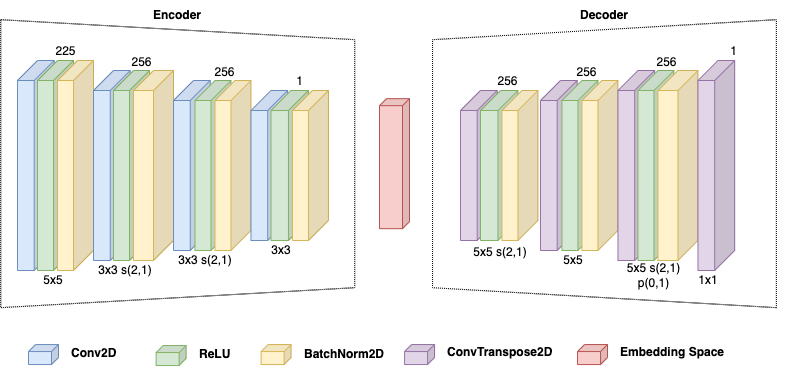
\includegraphics[width=\textwidth]{images/experiments/autoencoder_init.png}
\end{figure}

\newpage
\subsubsection{Evaluation}
Regarding the evaluation of this first model, it had been tested out on the remaining 20\% of the small subset. These first experiments consisted just of evaluating the outcome of the decoder, by passing single spectrograms through the network. By this, the ability of the network to recreate audio spectrograms was proven, which further on serves as a base for the next experiments. Regarding the final outcoming sounds, the original preserved phase information was reused to recreate audios.

\subsection{Spectrograms of signalframes as Input}
In the previous initial experiment, the samples from the NSynth dataset have been taken as a whole for the experiment. It has been mentioned that all samples are 4 seconds long, but some contain padding in order to reach a length of 4 seconds. As those zero-paddings are then also part of the training data, this could affect the behaviour but also the outcome of the model. If those zero-paddings would be left out, this would lead to unequal samples, which results in training data unusable for the model. This is because the network has a fixed size of neurons at the input, which implies to have a fixed input shape. Furthermore this also means that having a fixed size of 4 seconds, the input always has to be of 4 seconds, which is not desirable. Not at least, if the system should be used in real-time applications for audio synthesis, one cannot wait to have 4 seconds of a signal, to perform audio synthesis with it. Therefore it would be desirable to perform audio synthesis on smaller "frames or chunks" of an audio signal, respective spectrogram. 

\newpage
\subsubsection{Pre-processing}
This leads to the idea to take chunks or frames of audio data that get transformed into distinct spectrograms of same size. For a start the length of those frames was set to 500 ms. Furthermore it was chosen that those frames are not consecutive, but have an overlap of 50\%. Additionally those frames were multiplied with a window function, like it is used in the STFT. Similar to the window function used in the STFT, here a Hann-window is used. Again as those trimmed signals were all differently long, they had to be padded to a multiple of the frame size respective hop-length. This ensures to have equally long chunks of the signal. As of the windowed frames, the first and last frame didn't have overlapping parts at the beginning respective end. To overcome this issue, additional zeros were padded to form one frame on each side, to also get an overlap. In combination, having the framed and windowed signal chunks, by overlapping each again with 50\% and adding the values, this would yield the original signal again. This would be especially helpful when reconstructing the final signal in the end. 

Having those framed and windowed signal chunks, the STFT gets applied on those, having the same configuration as in the first experiment. This then leads to have multiple spectrograms for the length of 500 ms with again a frequency resolution of 31,25 Hz. Again for the training and testing, additional to the log-mag data, the phase information, reference value and name of the sample including a number to identify the frame got preserved for later use.

\subsubsection{Model and training}
The configuration of the model is rather similar to the one used in the first setting. It has the same amount of layers on each side, despite different strides, but also different kernel-sizes got applied (see figure \ref{fig:cae_2D_init}). Again this one has been trained on 80\% of the \textit{keyboard\_synthetic} test dataset samples. Of course the significant difference here is, that now the input data are not whole spectrograms but overlapping frames. This also means that the amount of data has increased. When collecting the spectrograms for the dataset, the names get shuffled, in order to not have the same order. In contrast, the single frames don't get shuffled during training. Again the training has been performed over 20 epochs on the local machine.

\subsubsection{Testing/Evaluation}
For the purpose of evaluating the test score this has been done with the remaining 20\% of the samples. To evaluate the ability of the autoencoder to reconstruct spectrograms, the whole samples were used including those from the training. Here the spectrograms were provided in the order as they appear. Having all reconstructed spectrograms, the inverse STFT was applied with the preserved phase information. Resulting in the frames corresponding to every single input note, those got overlapped and added (in their right order). By this procedure the signal with the original length could be obtained and further on evaluated auditorily. For results see chapter \ref{cha:Results}. 

A step for interpolating two different sources has not been investigated here, up to these experiments. Also the embedded space also has not been evaluated so far but will be subject of further experiments.

\section{Experiments single frequency vectors}
The above mentioned experiments, were a proof regarding the ability of convolutional autoencoders to recreate audio spectrograms. From this point on the experiments were done using the whole training dataset and also include audio synthesis. In the previous experiment the model was trained on frames of audio data which were 500 ms long. Having the idea to synthesise audio on real-time input, this would mean that always a signal frame of 500 ms has to be present, in order to have an input for the model. Therefore it is desirable to have an input that is as short as possible. An important note at this point is therefore, that spectrograms consist of frequency by time data. Each vector of the spectrogram along the time axis represents a short frame of time. 

As mentioned before, when pre-processing was done on 16 kHz sampled data with an \texttt{n\_fft} of 512, respective \texttt{hop-length} of 256, a time resolution of 16 ms was therefore present. Therefore the idea was to take those single frequency vectors as input for the model. The shape therefore is frequency by channels which in the case of the previous parameters is 256x1. Having this idea, also the silence at the end of the signals could be omitted as just the frequency domain was used for the models input. This therefore enabled taking samples of different length in time. Throughout the experiment the value for the \texttt{n\_fft} was increased to 1024, as an increase of the models performance could be achieved. Increasing this parameter therefore meant to decrease the time resolution, but increased the amount of frequency bins and thus having a better frequency resolution. Resulting in a number of 513 frequency bins (15,625 Hz/bin) and time resolution of 32ms per vector.


\subsubsection{Neural network}
As a consequence a different model had to be used, as 2D convolutions were no more suited. Therefore a model was designed that uses 1D convolutions. 1D convolutions are performing the same calculations, with the difference of having just a 1-dimensional kernel. This one dimensional kernel just operates on the frequency axis and tries to extract important features. Equally to the 2D convolutions they also apply the principle of channels. Regarding the channels, those also get expanded but then subsequently until the innermost layer reduced to 1 in order to form a single dimensional vector. Until the end again those channels get expanded but reduced again to 1 to have the same shape as the input vector. In figure \ref{fig:cae_1D}, the structure and configuration of this autoencoder is depicted. 

 \begin{figure}[htb!]
	\caption{Deep 1D convolutional autoencoder.}
	\label{fig:cae_1D}
	\centering
	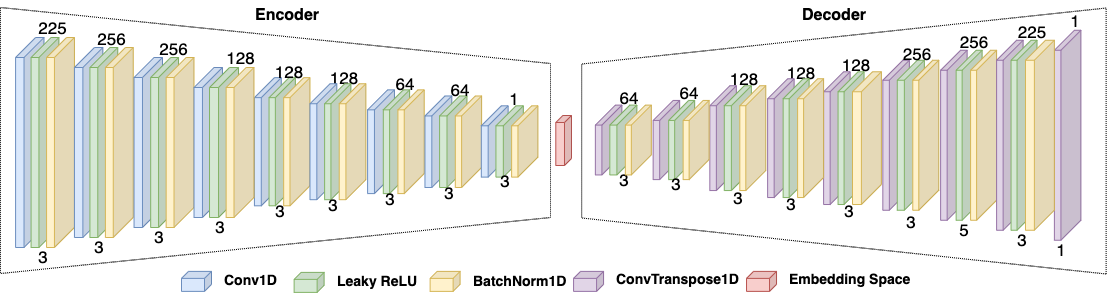
\includegraphics[width=\textwidth]{images/experiments/autoencoder_deep_1D.png}
\end{figure}


\subsubsection{Training}
The training process for this experiment differs in some major points from the previous ones. The main difference lies in the shape of the data. This can be concluded as here just the single frequency vectors were used for this network and therefore the network itself has 1D convolutions as discussed before. Furthermore, this experiment was originally trained locally with the small subset like before, but later on, access to a GPU-accelerated instance was made available. This GPU instance, as discussed at the beginning of this chapter, enabled training complex ML models with a large amount of data, over a long time. With this possibility, the full training dataset could be utilized as it consists of several thousands of audio samples and would be too big to use locally. This does not mean that the whole dataset was used all the time for training on this instance. With the progress of the project, several trainings with different amounts of data were made, that impacted the training process.

% \begin{itemize}
%     \item \textbf{Single Instrument}
%     \item \textbf{Multiple Instruments (>=2)}
%     \item \textbf{All Instruments}\\
% \end{itemize}

%\noindent
%Regarding the training performance, some interesting findings and observations could be made which get mentioned when showing the results. 

As here single frequency vectors were used, the process of creating a tensor and subsequently the dataset for the dataloader, was different. Here all spectrograms of the pre-defined and pre-processed dataset were utilized, and the single frequency vectors get concatenated to form one big 3D array in the shape of amount by channels by frequency. To note the amount of channels here is also initially one. While experimenting, regarding the training, also different strategies regarding shuffling were used. First on just the samples were shuffled resulting in the instruments being mixed, but the frequency vectors were in the same order as in the spectrogram. This stayed the same as after each epoch the data didn't get shuffled. One more successful strategy was to also shuffle the whole generated array, resulting in the frequency vectors of all instruments being mixed. Furthermore shuffling was also done after each epoch. The same strategies were also applied to the validation dataset, as from this point on also the validation dataset was considered, partly due to more computational power was present from this point on. A batch-size of 32 was considered. 

Introducing the validation step from this experiment, also the scheduler to adapt the learning rate during the training was applied. Taking into account that the network is rather complex and a huge amount of data has been used, the learning rate also had to be chosen adequately. Throughout these experiments, a small learning rate of $1e-7$ was chosen, as this led to a more stable training and better convergence. 

\subsubsection{Testing}
As described above, after each training, the current model state was saved, those can be used for the testing and evaluation regarding synthesis. As having numerous states that got saved, the one with the lowest error score on the validation set got considered for further steps. For the steps around testing and evaluation, the held-out test dataset was used. This stage was configured to either take the whole test dataset, a specific pitch, or a specific instrument source. By this technique its made possible to get the scores and therefore performance for certain instruments or pitch. 

\subsection{Experiments for Synthesis}
Having this kind of network that was trained on the training dataset, to reconstruct single frequency vectors, some experiments have been conducted for generating audio. As during the training the network learned how to reconstruct frequency vectors, one experiment is to examine the quality of the output for a single non-modified audio. Those are similar to the ones conducted in the first experiments above. Also by reconstructing just single notes, the preserved phase information could be reused, which enabled application of the ISTFT. For a comparison also the Griffin-Lim algorithm was utilized.

As the main objective of this work was to examine the capability of creating novel sounds, from this point on in the project the interpolation step was introduced. With the interpolation step the encoded features in the embedded space of two instruments were taken and value-wise interpolated. As it is known at this point, the encoder part of this network takes as input a vector of 513x1 and creates a lower-dimensional representation of it with the size of 495x1. Those representations can be seen as the essential features, and were considered for the interpolation task. For this task, the frequency vectors of two instruments of probably the same pitch were passed through the network. Here the data did not get shuffled, as it was important to produce the values in the same order as they come from the spectrograms. The output of the encoder for each instrument was concatenated to a 2D array 495x$N$ where $N$ is the number of encoded frequency vectors. To get a better idea of this concept, figure \ref{fig:exp_spec_emb_int_1D} shows two spectrograms with the corresponding accumulated output of the encoder.\\ 

 \begin{figure}[htb!]
	\caption{Input spectrograms with embeddings and interpolated embedding.}
	\label{fig:exp_spec_emb_int_1D}
	\centering
	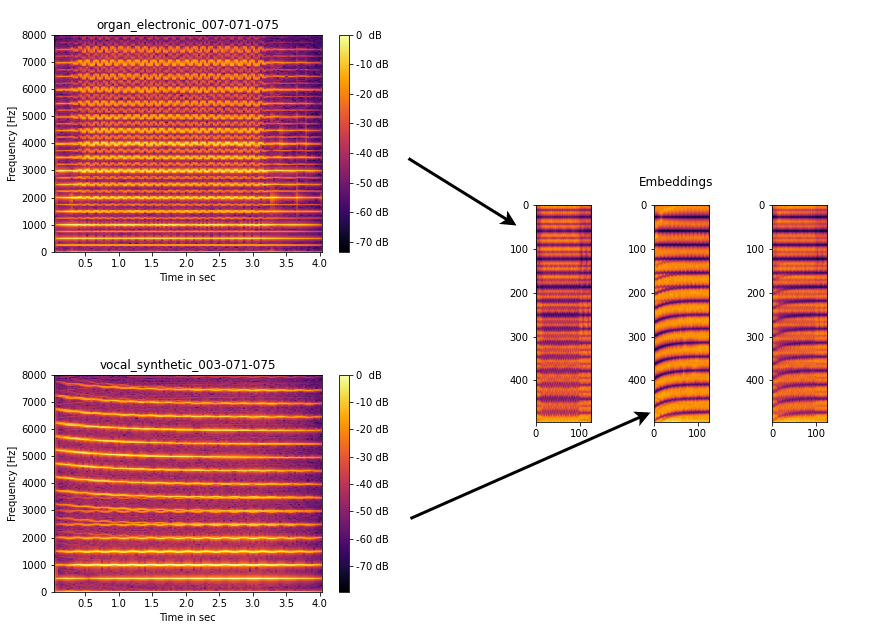
\includegraphics[width=\textwidth]{images/experiments/spec_to_emb.png}
\end{figure}

Having those two representations, interpolation was performed. Like discussed in chapter \ref{cha:Approach}, along the x-axis each output vector of one sample was interpolated with the corresponding output vector of the second sample. This process is also shown in figure \ref{fig:exp_spec_emb_int_1D} where the result of the interpolation process is shown. This process got applied equally for each subsequent experiments as the encoder output is always of the same shape, but more on that later on.
This interpolated vector was subsequently passed through the decoder part which forms again frequency vectors of 513x1 that were accumulated to a spectrogram. This spectrogram then depicts the result of audio synthesis combining features of two different instruments.

Further on this spectrogram was converted back to audio domain. As in this case no phase information is present, the Griffin-Lim algorithm \cite{Griffin1984} for phase estimation was applied. By listening to the final sound, it should be possible to hear the characteristics of both instruments combined in this sound.

\section{Experiments with slices of spectrograms}
\label{sec:exp_spec_slice}
Based on the results and insights that could be gained with the previous experiments (see chapter \ref{cha:Results}) some more experiments were made. Not at least to examine how different representations of the input data and as a consequence different model configurations influence the task of neural audio synthesis. For this case the following experiments in contrast worked with 2D representations as input. 2D data has already been used in the initial experiments with the whole spectrograms, but also spectrograms based on frames of the audio signal. As a difference for the following experiments, the spectrograms have been taken, but sliced into overlapping chunks. The spectrograms taken in this experiment were generated with the same configurations as in the previous experiment (\texttt{n\_fft=1024}, \texttt{hop\_length=512}). The idea to use chunks of spectrograms as input arose to improve the models performance with regard to synthesis and recreation of spectrograms. As by using single frequency vectors, just the frequency information is present and no information about its change over time. As a theory to also incorporate the temporal axis as input, important information about the temporal frequency changes could be captured. Those frequency changes could deliver more important characteristics of the samples that could be extracted. As not the whole spectrograms should be used as input, chunks of them are favorable, to keep the input as small as possible. Therefore the choice has been made to take three consecutive frequency vectors to form a frame with the shape of (513x3). Throughout the experiments it has been tried out to either take the frames subsequently or overlapping, leading to the preference in taking the latter. The overlap has chosen to be always 2 vectors from the preceding frame. 

For demonstration, let there be a spectrogram $spec=[f_0, f_1, f_2, f_3, f_4, f_5, ... f_n]$ of length $n$ where $f_i$ is the frequency vector at index $i$. This results in an array of $specs\_slices=[[f_1, f_2, f_3], [f_2, f_3, f_4], [f_3, f_4, f_5] ... [f_{n-3}, f_{n-2}, f_{n-1}], [f_{n-2}, f_{n-1}, f_n]]$. The idea behind this overlap was to capture every change or time-pattern in the source spectrogram. This technique also had the advantage that all the silence of the source spectrograms could be cut away, allowing to use differently long spectrograms as input. A positive side-effect here was also to gain additional input data, on which the model could be trained on. As the models output are also overlapping frames, to reconstruct the final spectrogram and audio, this also had to be considered, but more on that later on. Again when creating the tensor and dataset, the spectrograms were taken in a random order. At first the resulting frames of the training set didn't get shuffled. Later on during the training, the frames in the batches, which again are of size 32, were shuffled like in previous examples. The same happened to the validation dataset, while it also was shuffled initially and after each epoch. An important note is that for the training and validation the whole dataset were used all the time. 

\subsubsection{Neural Network}
As again input data in a 2D shape was used for these experiments, the model again had to be adapted. Instead of 1D convolutions and 1D batch normalization again, 2D convolutions and 2D batch normalization has been used. Also in contrast to the previous network, a normal ReLU activation has been used. These experiments incorporate different model configurations whereas a special focus has been given to the amount of striding and thus input compression. Here it should be evaluated, how more compression and thus a smaller latent space influences the quality of the decoder output and further on of the generated audio. Both in terms of single note reconstruction and interpolation based synthesis. The following figure \ref{fig:exp_2D_cae} shows, the basic network structure for these kinds of experiments.

 \begin{figure}[htb!]
	\caption{2D convolutional autoencoder.}
	\label{fig:exp_2D_cae}
	\centering
	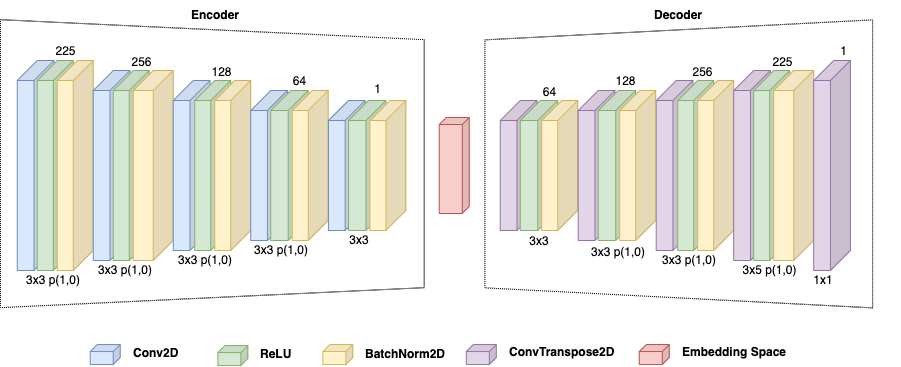
\includegraphics[width=\textwidth]{images/experiments/autoencoder_2D.png}
\end{figure}

This network is not as deep as the one used in the previous experiment because it consists of 5 layers on each side (10 in total). As the input is of size 513x3, the convolutions had to use a padding along the time axis. If no padding would be applied, just one time a kernel of 3x3 could be applied. Thus 5 times a 3x3 kernel could be applied with the last layer having no padding. This results in a single 1D vector in the embedded space. In the decoder part, padding also had to be applied to regain the same dimensionality in the end. As previously said, these experiments should give an insight on how the striding and thus the size of the embedding influences the performance and quality of the output. Choosing more strides and a smaller embedding, the network has to learn to extract more efficient encodings, from which it can reconstruct the input data. Thus by choosing a small embedding size, the network should learn to extract the most important features of the input. Therefore the size is also of significance regarding the audio synthesis task by interpolating the embeddings. In the following table \ref{tab:exp_2D_strides}, the different configurations regarding the striding are shown. 


\begin{table}[htb!]
    \centering
    \begin{tabular}{|c|c|c|c|}
        \hline
         &\textbf{Encoder}&\textbf{Embedding-size}&\textbf{Decoder} \\
         \hline
        \textbf{Single-Stride} & e2 & 250 & d4 \\
        \hline
        \textbf{Double-Stride} & e2, e4 & 124 & d2, d4 \\
        \hline
        \textbf{Triple-Stride} & e2, e3, e5 & 62 & d1, d3, d4 \\
        \hline
    \end{tabular}
    \caption{Setting of strides in network.}
    \label{tab:exp_2D_strides}
\end{table}

To explain, each row represents a network configuration, that either uses one, two or three times a striding of (1,2) on each side of the network. As of the shape of the input, striding can just be applied on the frequency axis. The columns with the names "Encoder" and "Decoder" show the respective layers where the stride was applied. For example e2 is the second layer in the Encoder and d4 the fourth layer in the decoder. The center column called "Embedding-size" explains the size of the embedded space vector. By having these model configurations, interesting findings and results could be obtained. 

\subsection{Audio synthesis}
In the previous experiment with the 1D convolutional network, the interpolation step has been introduced. This step was also applied with this network. As the embedded space vector also has the shape of a 1D vector, the interpolation procedure here was exactly the same. 

\subsubsection{Analysis of the embedded space}
As with neural audio synthesis novel interesting sounds should get generated, it is also of interest to find interesting combinations for the interpolation. Combined with the fact that the embeddings contain the extracted features/characteristics of a sound, those can be utilized for this task. It therefore has been implemented to take the output of the encoder of several notes (e.g. from the same pitch) and compute the correlation coefficients between those. The result got depicted in a correlation matrix to see which samples have the lowest correlation coefficients. Low correlation coefficients between two data samples mean that those have little similarities and thus different characteristics. By taking those embeddings with the lowest correlation coefficients and interpolating them, interesting novel sounds can be generated. More on that in the next chapters.

\subsection{Reconstruction and post-processing}
\label{subsec:exp_rec_post}
As the shape of the output of the network is also the same as of the input of the network, this had to be considered when recreating the spectrogram. The output therefore were also again frames of 3 that had to be overlapped. During the experiments different strategies have been tried out, whereas it was preferred to average the overlapping parts of the output frames, in order to form the final spectrogram.

When having the final spectrograms, some further experiments regarding the improvement of the sound quality have been carried out. In this case this includes to correct energy in the frequency bands of the output. With this technique important properties of the sound like the transient or impulse (e.g. guitar stroke) should be preserved. For this task in advance the energy-values of the frequencies were summed up for each frequency vector of the original audio spectrograms. This was also done for the output spectrogram and its frequency vectors, after converting from dB to energy. By comparing those sums with the corresponding values of the input spectrogram, a factor could be calculated. This factor then was multiplied with the corresponding output frequency vector in order to have the same amount of energy present in the output spectrogram. If the output spectrogram was generated by an interpolated embedding, the energy sums of the two input samples were taken and averaged. These averaged values then were taken as a reference to correct the energy. By performing the inverse STFT or Griffin-Lim algorithm, the resulting audio sample should therefore also have a corrected amplitude and thus improved sound. Regarding the results, those will be discussed as well later on in the thesis.


\section{Experiments with mel scale}
\label{sec:exp_mel}
Up to this point, the experiments have all been conducted on log-magnitude spectrograms. Those spectrograms depict the frequency energies on a linear scale with a certain resolution (e.g. [0 Hz, 15,625 Hz, 31,25 Hz ... 8000 Hz]). Those spectrograms have been computed of a dataset consisting of musical notes. Those notes can be grouped into musical intervals describing the distance of a note to another, whereas the interval of an octave would be a doubling in frequency. As an example the note \textit{a'} has a frequency of 440 Hz (if perfect sine), whereas its octave on top would be an \textit{a''} with 880 Hz. If going an octave down it would result in 220 Hz having an \textit{a} (to be continued \textit{A} 110 Hz, \textit{A'} 55 Hz, ...). This also means that the higher the note gets, the larger the distance in Hz and the lower it gets, the less distance in Hz between the notes. Having this principle one can come to the conclusion that having a linear scale like in log-magnitude spectrograms, the resolution with lower notes is worse then with higher notes. With a look onto machine learning and neural networks, this also means, that there is less data available to train on for low notes.
Keeping this in mind, the choice has been made to perform comparative experiments based on a different scale, which is called mel scale \cite{stevens1937scale}. This scale can be seen as a compressed form of a spectrogram. Furthermore it is an empirical scale that is based on the human auditory perception, as they perceive frequency logarithmically rather than linearly. Mapped on the mel scale, in contrast to magnitude, low-frequency contents have a better resolution in contrast to the high-frequency range \cite{Kathania2019}. This means that with this scale lower notes can be better differentiated and thus are more emphasized then with the linear scale. Even though that this scale is based on observations it was proven to be beneficial regarding machine learning tasks. Not at least as several approaches, mentioned in related work, applied this scale for their audio synthesis task. Furthermore this scale could also be seen as a compressed form of a spectrogram containing the most significant properties. 

\subsection{Pre-processing}
The pre-processing step does not really differ from the ones performed in previous experiments. A difference here is in order to obtain spectrograms with the mel scale to call the \textit{librosa} function \texttt{librosa.feature.melspectrogram()} which takes as input a pre-computed STFT-spectrogram. Throughout this experiment the spectrograms created with an \texttt{n\_fft} of 1024 and \texttt{hop\_length} of 512 have been taken to be converted to mel-spectrograms. The resulting mel-spectrogram has a size of 128x$t$ and thus is smaller than the mag-spectrogram (513x$t$). Having the mel-spectrograms the same steps as with log-magnitude were performed (dB conversion, preserving the power reference, ...). Also for the model training, frames of 3 vectors of the mel-spectrogram were taken as input for the model. In the next figure \ref{fig:exp_mag_mel} a mel-spectrogram with its corresponding log-magnitude spectrogram is displayed, to see the difference.

\begin{figure}[htb!]
    \centering
    \makebox[\textwidth][c]{\begin{tabular}{@{}c}
        \makebox{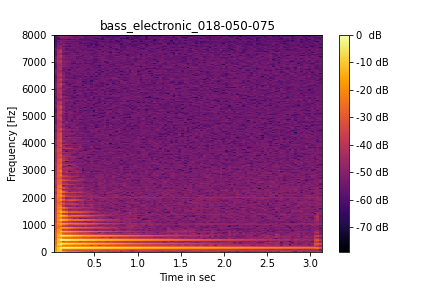
\includegraphics[width=0.55\textwidth]{images/experiments/bass_electronic_log-mag.png}}\\
        log-mag spectrogram ~(a)\\
        \makebox{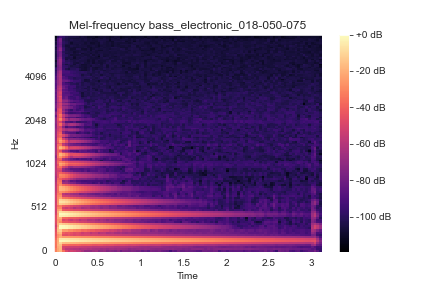
\includegraphics[width=0.55\textwidth]{images/experiments/bass_electronic_log-mel.png}}\\
        log-mel spectrogram ~(b)
    \end{tabular}}
    \caption{Difference between log-magnitude and log-mel spectrograms.}
    \label{fig:exp_mag_mel}
\end{figure}

By comparing those, it can be seen, that the scale is logarithmic and the distance between the low frequencies greater than between the high-frequencies. As of this known characteristics and its already compressed form, the experiments using these kind of spectrograms thus can be expected to bring different but interesting results. Here also the same experiments with and without interpolation got conducted to get a comparison.

\subsubsection{Neural Network}
Like in the previous experiment, also three different networks with single-, double- or triple-strides on each side were applied and assessed further on. The basic network structure and configuration does not differ of the one used in the previous experimental setting as having the same amount of layers and same configuration of the channels. Nevertheless some differences arise, because the last layer applies a kernel of 1x2 to regain the same input shape. Also in the networks using three or two times strides on each side, padding in the layer \textit{e4} and \textit{d4} is set to 1,1. Regarding the network with three strides on each side, those have been set onto layers \textit{e2, e3, e4} and \textit{d2, d3, d4}. As the input of the network is already of smaller size, the corresponding embeddings are therefore significantly smaller like in the previous experiments (56, 28, 14). Those were also altered like in the previous experiments by interpolation to synthesize novel sounds. 

\subsubsection{Reconstruction and post-processing}
The steps around the reconstruction and post-processing are similar to the previous experiments. Because as input also frames of 3 were used, the output consists of 3 frames too. Those also were overlapping and averaged to form a final log-mel spectrogram. Again also the energy got corrected to have the same amount of energy present like in the input. Having the final log-mel spectrograms, those could be either directly converted to an audio using the function \texttt{librosa.feature.inverse.mel\_to\_audio} or first to an magnitude spectrogram. The latter is used when just single audio samples were reconstructed (without interpolation) as here the phase information could be reused, and thus the ISTFT can be applied to obtain the final sound. Otherwise the mentioned function is performing the conversion to magnitude and Griffin-Lim at once to obtain an estimated signal. 


